\documentclass[12pt]{article}
\usepackage[margin=1in]{geometry}
\usepackage{setspace}
\onehalfspacing

% Start of preamble
%==========================================================================================%
% Required to support mathematical unicode
\usepackage[warnunknown, fasterrors, mathletters]{ucs}
\usepackage[utf8x]{inputenc}

\usepackage[dvipsnames,table,xcdraw]{xcolor}

% Standard mathematical typesetting packages
\usepackage{amsmath,amssymb,amscd,amsthm,amsxtra, pxfonts}
\usepackage{mathtools,mathrsfs,dsfont,xparse}

% Symbol and utility packages
\usepackage{cancel, textcomp}
\usepackage[mathscr]{euscript}
\usepackage[nointegrals]{wasysym}
\usepackage{apacite}

% Extras
\usepackage{physics}  
\usepackage{tikz-cd} 
\usepackage{microtype}
\usepackage{enumitem}
\usepackage{titling}
\usepackage{graphicx}

% Fancy theorems due to @intuitively on discord
\usepackage{mdframed}
\newmdtheoremenv[
backgroundcolor=NavyBlue!30,
linewidth=2pt,
linecolor=NavyBlue,
topline=false,
bottomline=false,
rightline=false,
innertopmargin=10pt,
innerbottommargin=10pt,
innerrightmargin=10pt,
innerleftmargin=10pt,
skipabove=\baselineskip,
skipbelow=\baselineskip
]{mytheorem}{Theorem}

\newenvironment{theorem}{\begin{mytheorem}}{\end{mytheorem}}

\newtheorem{corollary}{Corollary}
\newtheorem{lemma}{Lemma}

\newtheoremstyle{definitionstyle}
{\topsep}%
{\topsep}%
{}%
{}%
{\bfseries}%
{.}%
{.5em}%
{}%
\theoremstyle{definitionstyle}
\newmdtheoremenv[
backgroundcolor=Violet!30,
linewidth=2pt,
linecolor=Violet,
topline=false,
bottomline=false,
rightline=false,
innertopmargin=10pt,
innerbottommargin=10pt,
innerrightmargin=10pt,
innerleftmargin=10pt,
skipabove=\baselineskip,
skipbelow=\baselineskip,
]{mydef}{Definition}
\newenvironment{definition}{\begin{mydef}}{\end{mydef}}

\newtheorem*{remark}{Remark}

\newtheorem*{example}{Example}

% Common shortcuts
\def\mbb#1{\mathbb{#1}}
\def\mfk#1{\mathfrak{#1}}

\def\bN{\mbb{N}}
\def \C{\mbb{C}}
\def \R{\mbb{R}}
\def\bQ{\mbb{Q}}
\def\bZ{\mbb{Z}}
\def \cph{\varphi}
\renewcommand{\th}{\theta}
\def \ve{\varepsilon}
\newcommand{\mg}[1]{\| #1 \|}

% Often helpful macros
\newcommand{\floor}[1]{\left\lfloor#1\right\rfloor}
\newcommand{\ceil}[1]{\left\lceil#1\right\rceil}
\renewcommand{\qed}{\hfill\qedsymbol}
\renewcommand{\P}{\mathbb P\qty}
\newcommand{\E}{\mathbb{E}\qty}
\newcommand{\Cov}{\mathrm{Cov}\qty}
\newcommand{\Var}{\mathrm{Var}\qty}

% Sets
\usepackage{braket}

\graphicspath{{/}}
\usepackage{float}

\newcommand{\SET}[1]{\Set{\mskip-\medmuskip #1 \mskip-\medmuskip}}

% End of preamble
%==========================================================================================%

% Start of commands specific to this file
%==========================================================================================%

\usepackage{listings}
\lstset{
  columns=flexible,
  basicstyle=\small\ttfamily,
  mathescape=true,
  escapeinside=||
}
\usepackage{subcaption}

%==========================================================================================%
% End of commands specific to this file

\title{CSE Template}
\date{\today}
\author{Rohan Mukherjee}

\begin{document}
    \maketitle
    \subsection*{1.1.3}
    \begin{enumerate}
        \item I think the main reason cosine similarity works better than other distance metrics like L1/L2 is because it is norm-invariant. If you have two sentence embeddings $x$ and $y$, and these were really similar, one would expect that $2x$ and $2y$ would be really similar too. In fact, you would think these would be just as similar as $x$ and $y$. This is only true for cosine similarity. 
        \item It chooses option a, pessimistic, instead. Recall that the Glove representation we are using for words is the context based wordvec model. Although positive and sanguine are synonyms, it is more likely that pessimistic has a context more simliar to sanguine than to pessimistic. Of course these words are similar, being antonyms, and there is no way to tell the difference between synonyms and antonyms with Glove. 
        \item I created the following questions:

        \textbf{Question 1:} Relation: Present to Past Tense \\
        Go is to went as eat is to \underline{\hspace{2cm}}?

        \begin{enumerate}
            \item[a)] \fbox{ate}
            \item[b)] gone
            \item[c)] going
            \item[d)] eaten
        \end{enumerate}

        \textbf{Question 2:} Relation: Present to Past Tense \\
        Walk is to walked as run is to \underline{\hspace{2cm}}?

        \begin{enumerate}
            \item[a)] \fbox{ran}
            \item[b)] running
            \item[c)] walk
            \item[d)] walks
        \end{enumerate}

        \textbf{Question 3:} Relation: Sequence Order \\
        5 is to 4 as 3 is to \underline{\hspace{2cm}}?

        \begin{enumerate}
            \item[a)] \fbox{2}
            \item[b)] 1
            \item[c)] 0
            \item[d)] -1
        \end{enumerate}

        \textbf{Question 4:} Relation: Sequence Order \\
        One is to two as three is to \underline{\hspace{2cm}}?

        \begin{enumerate}
            \item[a)] \fbox{four}
            \item[b)] five
            \item[c)] six
            \item[d)] seven
        \end{enumerate}

        \textbf{Question 5:} Relation: Country/Capital \\
        France is to Paris as Germany is to \underline{\hspace{2cm}}?

        \begin{enumerate}
            \item[a)] \fbox{Berlin}
            \item[b)] Munich
            \item[c)] Frankfurt
            \item[d)] Hamburg
        \end{enumerate}

        \textbf{Question 6:} Relation: Country/Capital \\
        India is to New Delhi as Japan is to \underline{\hspace{2cm}}?

        \begin{enumerate}
            \item[a)] \fbox{Tokyo}
            \item[b)] Kyoto
            \item[c)] Osaka
            \item[d)] Hiroshima
        \end{enumerate}

        \item First, here is the graph of the effect sizes vs vector sizes with the number of tokens fixed at 6B:
        \begin{figure}[H]
            \centering
            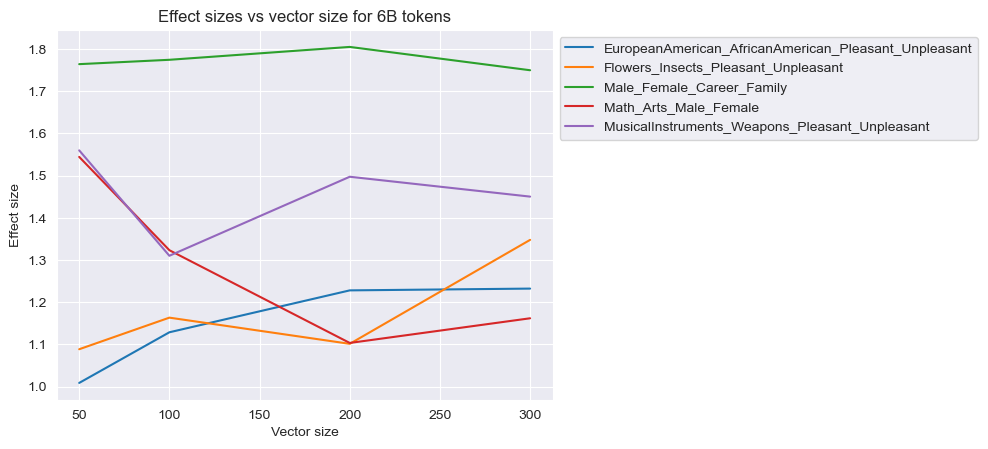
\includegraphics[width=0.8\textwidth]{images/effect_sizes_6b_tokens.png}
            \caption{Effect size vs Vector size}
        \end{figure}
        Here is the graph of the effect sizese vs number of tokens with vector size fixed at 300:
        \begin{figure}[H]
            \centering
            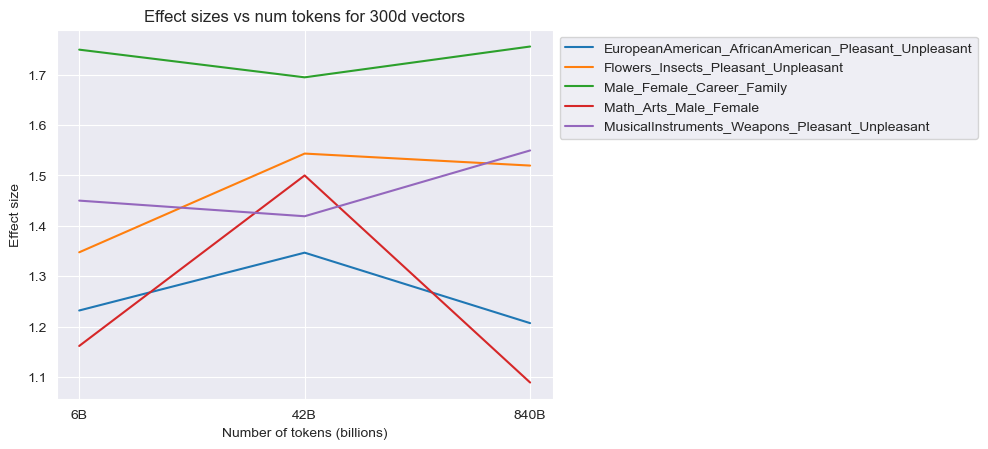
\includegraphics[width=0.8\textwidth]{images/effect_sizes_300d_vectors.png}
            \caption{Effect size vs Number of tokens}
        \end{figure}
        For both vector sizes and the number of tokens, the male female career family is held basically constant, same with musical instruments weapons. For math arts male female, the effect size drops as both the number of tokens and vector size increase. However, weirdly enough the middle token size of 42B it goes sharply up, then back sharply down. For the other two, they seem to increase at a slow rate. There isn't a clear trend, which is surprising. I am not surprised to see flower insect PUN to go straight up, as I feel like most people think of insects as gross, so that would be reflected in the graphs, which you can see in the number of tokens trained on.
    \end{enumerate}

    \newpage
    \subsection*{1.2.2}
    \begin{enumerate}
        \item The main problem is not understanding the context of our words. Due to not understanding context, the sentence "This movie is great and everyone who says otherwise is totally wrong, and abhorrent!" seems to be generally negative because it has a lot of negative words, but really isn't. Similarly, someone could say something like "This movie is great, but the second actor was bad". This would have the same sum as "This movie is bad, but the second actor is great", but these have different sentiments. 

        Also, using context-based embeddings is bound to run into issues with "The movie is bad" and "The movie is good", because good and bad have very similar contexts and so these would be very close together, when they should be far apart (and give opposite sentiments).
        \item Here is the graph of k vs accuracies:
        \begin{figure}[H]
            \centering
            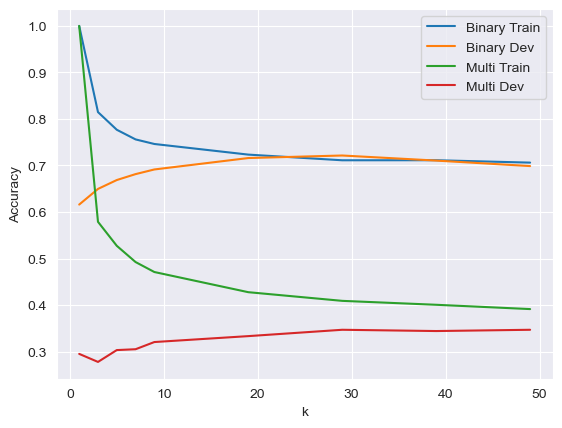
\includegraphics[width=0.8\textwidth]{images/effect_of_k_on_knn.png}
            \caption{k vs Accuracy}
        \end{figure}
        I notice that training accuracy moves consistently down, but the dev accuracy seems to increase up to a point. This is clear, as with k = 1 the model will just predict the same label because it has memorized the training data, and will do very bad on the dev data, as it hasn't. When k increases you get more generalizability, so the dev accuracy increases. But after a while, it gets gradually worse, as taking k to be the entire training set would always just output the same label. You would start comparing it to things that are not relevant. 
    \end{enumerate}

    \newpage
    \subsection*{2.2}
    \begin{enumerate}
        \item Say we set a max number of words of 2048. Then if we used padding instead of a sentence transformer, for the overwhemling majority of sentences, most of the words word be padding. This would mean that the overwhelming majority of our parameters would be useless most of the time, and the few times they are used they haven't been trained enough. So you would see a huge case of overfitting and poor generalizability. 

        This would likely also be extremely computationally expensive, as you would have to increase the number of parameters by probably an order of magnitude to account for the padding.

        \item Some of the issues I raised above happen when using the Glove representations vs sentence transformers. One notable example is: "And if you're not nearly moved to tears by a couple of scenes, you've got ice water in your veins." This follows almost the exact framework I said above: "This movie is (positive word) and if you disagree you are (negative word)". Of course the Glove reps would be confused because this is the same sentence as "This movie is (negative word) and if you disagree you are (positive word)". The sentence transformers would be able to understand the context of the words and would be able to differentiate between the two. The same logic applies to "The film serves as a valuable time capsule to remind us of the devastating horror suffered by an entire people." 

        \newpage
        \item

        For all these plots, both binary / multi class and siqa, I used the default hyperparameters of 
        \begin{itemize}
            \item lr = 1e-5
            \item epochs = 10
            \item batch size = 32
        \end{itemize}
        As in the spec, I used 1024 for depth experiments, and only 1 layer when testing the number of hidden units. 

        I got the following for binary and mulit-class case:

        \begin{figure}[H]
            \centering
        
            % First Row
            \begin{subfigure}{0.35\textwidth}
                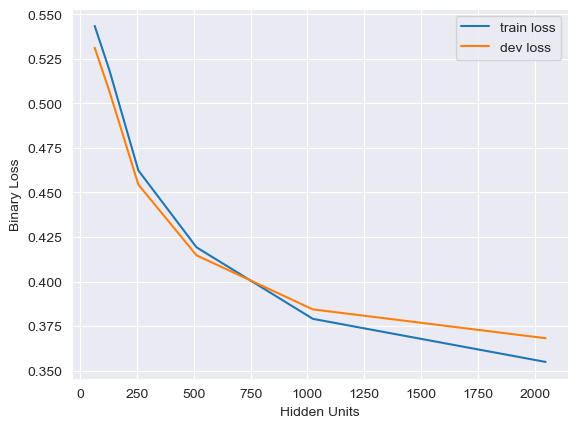
\includegraphics[width=\textwidth]{images/binary_units_loss.png}
                \caption{Binary - Units - Loss}
            \end{subfigure}
            \hfill
            \begin{subfigure}{0.35\textwidth}
                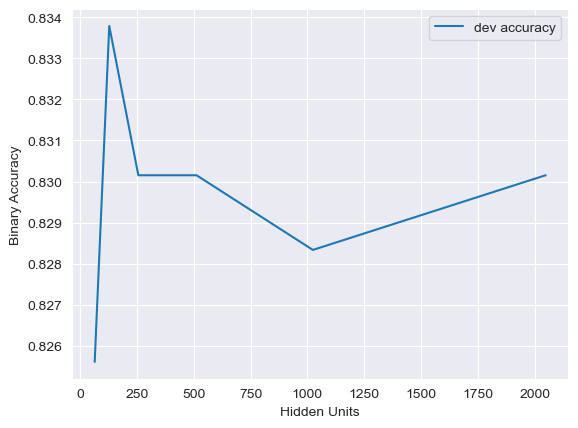
\includegraphics[width=\textwidth]{images/binary_units_acc.png}
                \caption{Binary - Units - Accuracy}
            \end{subfigure}
        
            % Second Row
            \begin{subfigure}{0.35\textwidth}
                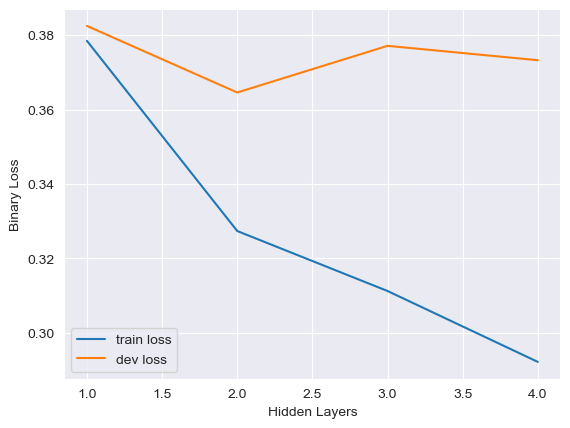
\includegraphics[width=\textwidth]{images/binary_layers_loss.png}
                \caption{Binary - Layers - Loss}
            \end{subfigure}
            \hfill
            \begin{subfigure}{0.35\textwidth}
                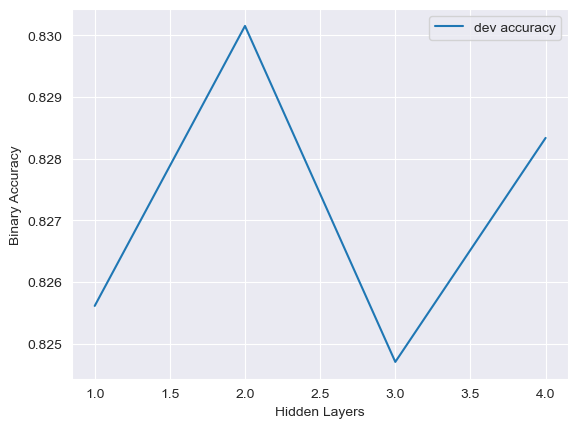
\includegraphics[width=\textwidth]{images/binary_layers_acc.png}
                \caption{Binary - Layers - Accuracy}
            \end{subfigure}
        
            % Third Row
            \begin{subfigure}{0.35\textwidth}
                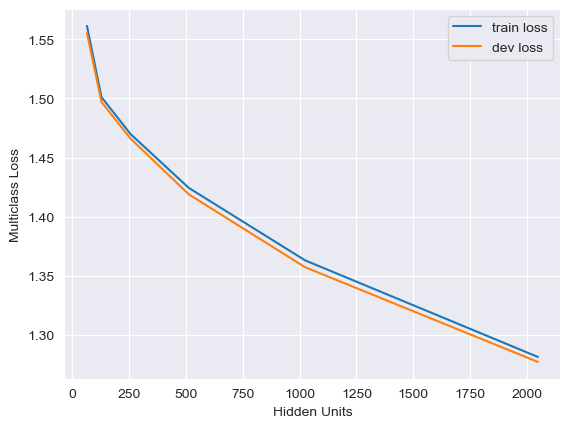
\includegraphics[width=\textwidth]{images/multi_units_loss.png}
                \caption{Multi - Units - Loss}
            \end{subfigure}
            \hfill
            \begin{subfigure}{0.35\textwidth}
                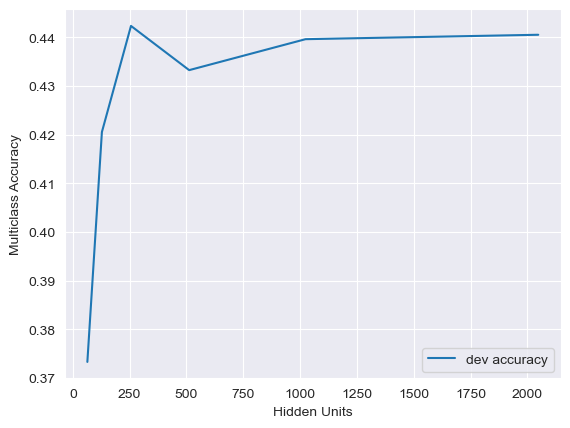
\includegraphics[width=\textwidth]{images/multi_units_acc.png}
                \caption{Multi - Units - Accuracy}
            \end{subfigure}
        
            % Fourth Row
            \begin{subfigure}{0.35\textwidth}
                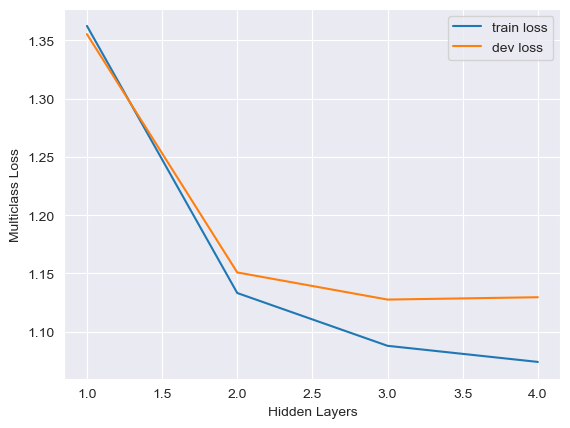
\includegraphics[width=\textwidth]{images/multi_layers_loss.png}
                \caption{Multi - Layers - Loss}
            \end{subfigure}
            \hfill
            \begin{subfigure}{0.35\textwidth}
                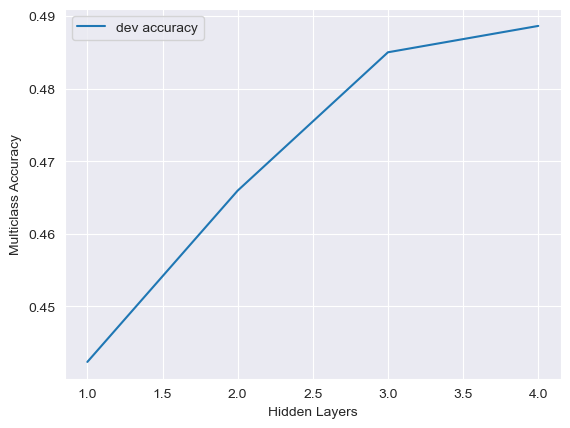
\includegraphics[width=\textwidth]{images/multi_layers_acc.png}
                \caption{Multi - Layers - Accuracy}
            \end{subfigure}
            \label{fig:graphs}
        \end{figure}

        It seems that generally, more units for the binary case is better, but somehow that doesn't translate to accuracy. This is probably because it starts to overfit. For the number of layers, the binary case doesn't do very well with more layers, since I think it isn't complex enough to merit more layers. The training loss goes down but the dev loss doesn't, and equivalently the accuracy is all over the place.

        For the multi-case, more units and more layers is better. I believe this is because the multi-class case is so complicated, that you really need a lot of parameters to accurately predict the sentiment, something the binary case does't need. 

        Here is the graph for SIQA:
        \begin{figure}[h!]
            \centering
        
            % Top Row (Units)
            \begin{subfigure}{0.45\textwidth}
                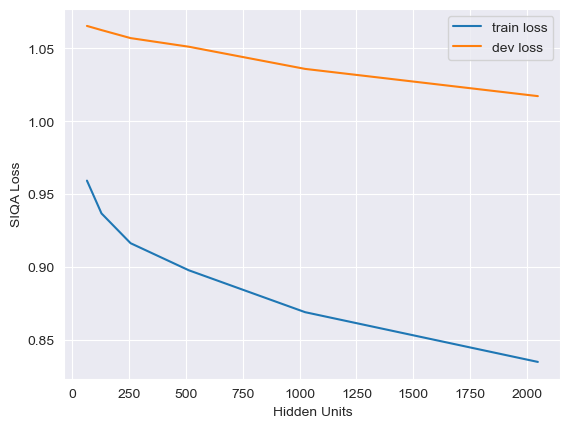
\includegraphics[width=\textwidth]{images/siqa_units_loss.png}
                \caption{SIQA - Units - Loss}
            \end{subfigure}
            \hfill
            \begin{subfigure}{0.45\textwidth}
                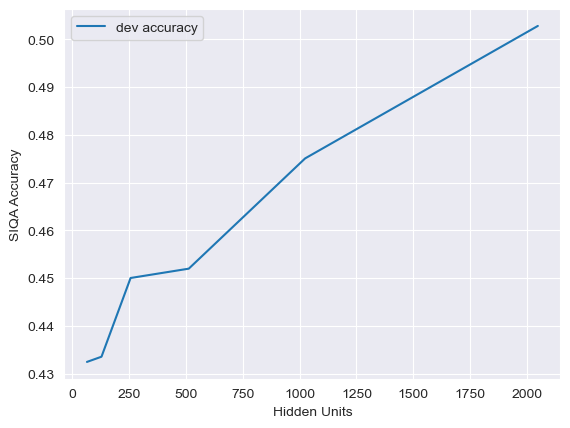
\includegraphics[width=\textwidth]{images/siqa_units_acc.png}
                \caption{SIQA - Units - Accuracy}
            \end{subfigure}
        
            % Bottom Row (Layers)
            \begin{subfigure}{0.45\textwidth}
                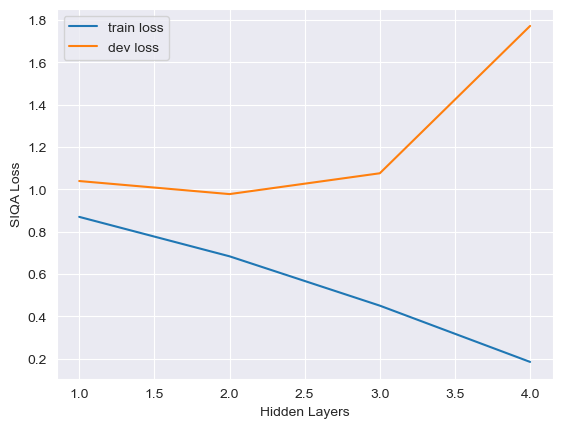
\includegraphics[width=\textwidth]{images/siqa_layers_loss.png}
                \caption{SIQA - Layers - Loss}
            \end{subfigure}
            \hfill
            \begin{subfigure}{0.45\textwidth}
                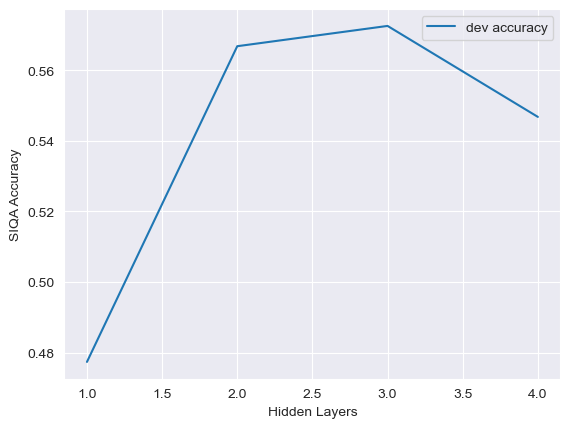
\includegraphics[width=\textwidth]{images/siqa_layers_acc.png}
                \caption{SIQA - Layers - Accuracy}
            \end{subfigure}
        
            \caption{SIQA results comparing units and layers configurations for loss and accuracy.}
            \label{fig:siqa_results}
        \end{figure}

        This one is less telling than the binary and multiclass case. For the number of hidden units, it seems that more units is better accuracy. However, the learning rate is also very small, and when I tested with learning rate of 1e-3, hidden units with 128 got an accuracy of 57\%, which is 14\% better than it did here. So I think that you need a lot more epochs to really get a full picture, but with 1e-5 it is clear that more units is better.

        For the number of layers, dev loss stays mostly constant but accuracy jumps by a lot, until 3 layers, when it starts to decrease. The same logic from before applies, to get a full picture you would need to test more hyperparameters, but for now it seems 3 layers is the best. I think this is because, like the last, the model starts overfitting after that, and the probablem is complicated enough to merit more layers. 

        \item I chose the Microsoft Research Paraphrase Corpus. I ended up training a simple Siamese Neural netowork, whose architecture is shown below (with layers=1):
        \begin{figure}[H]
            \centering
            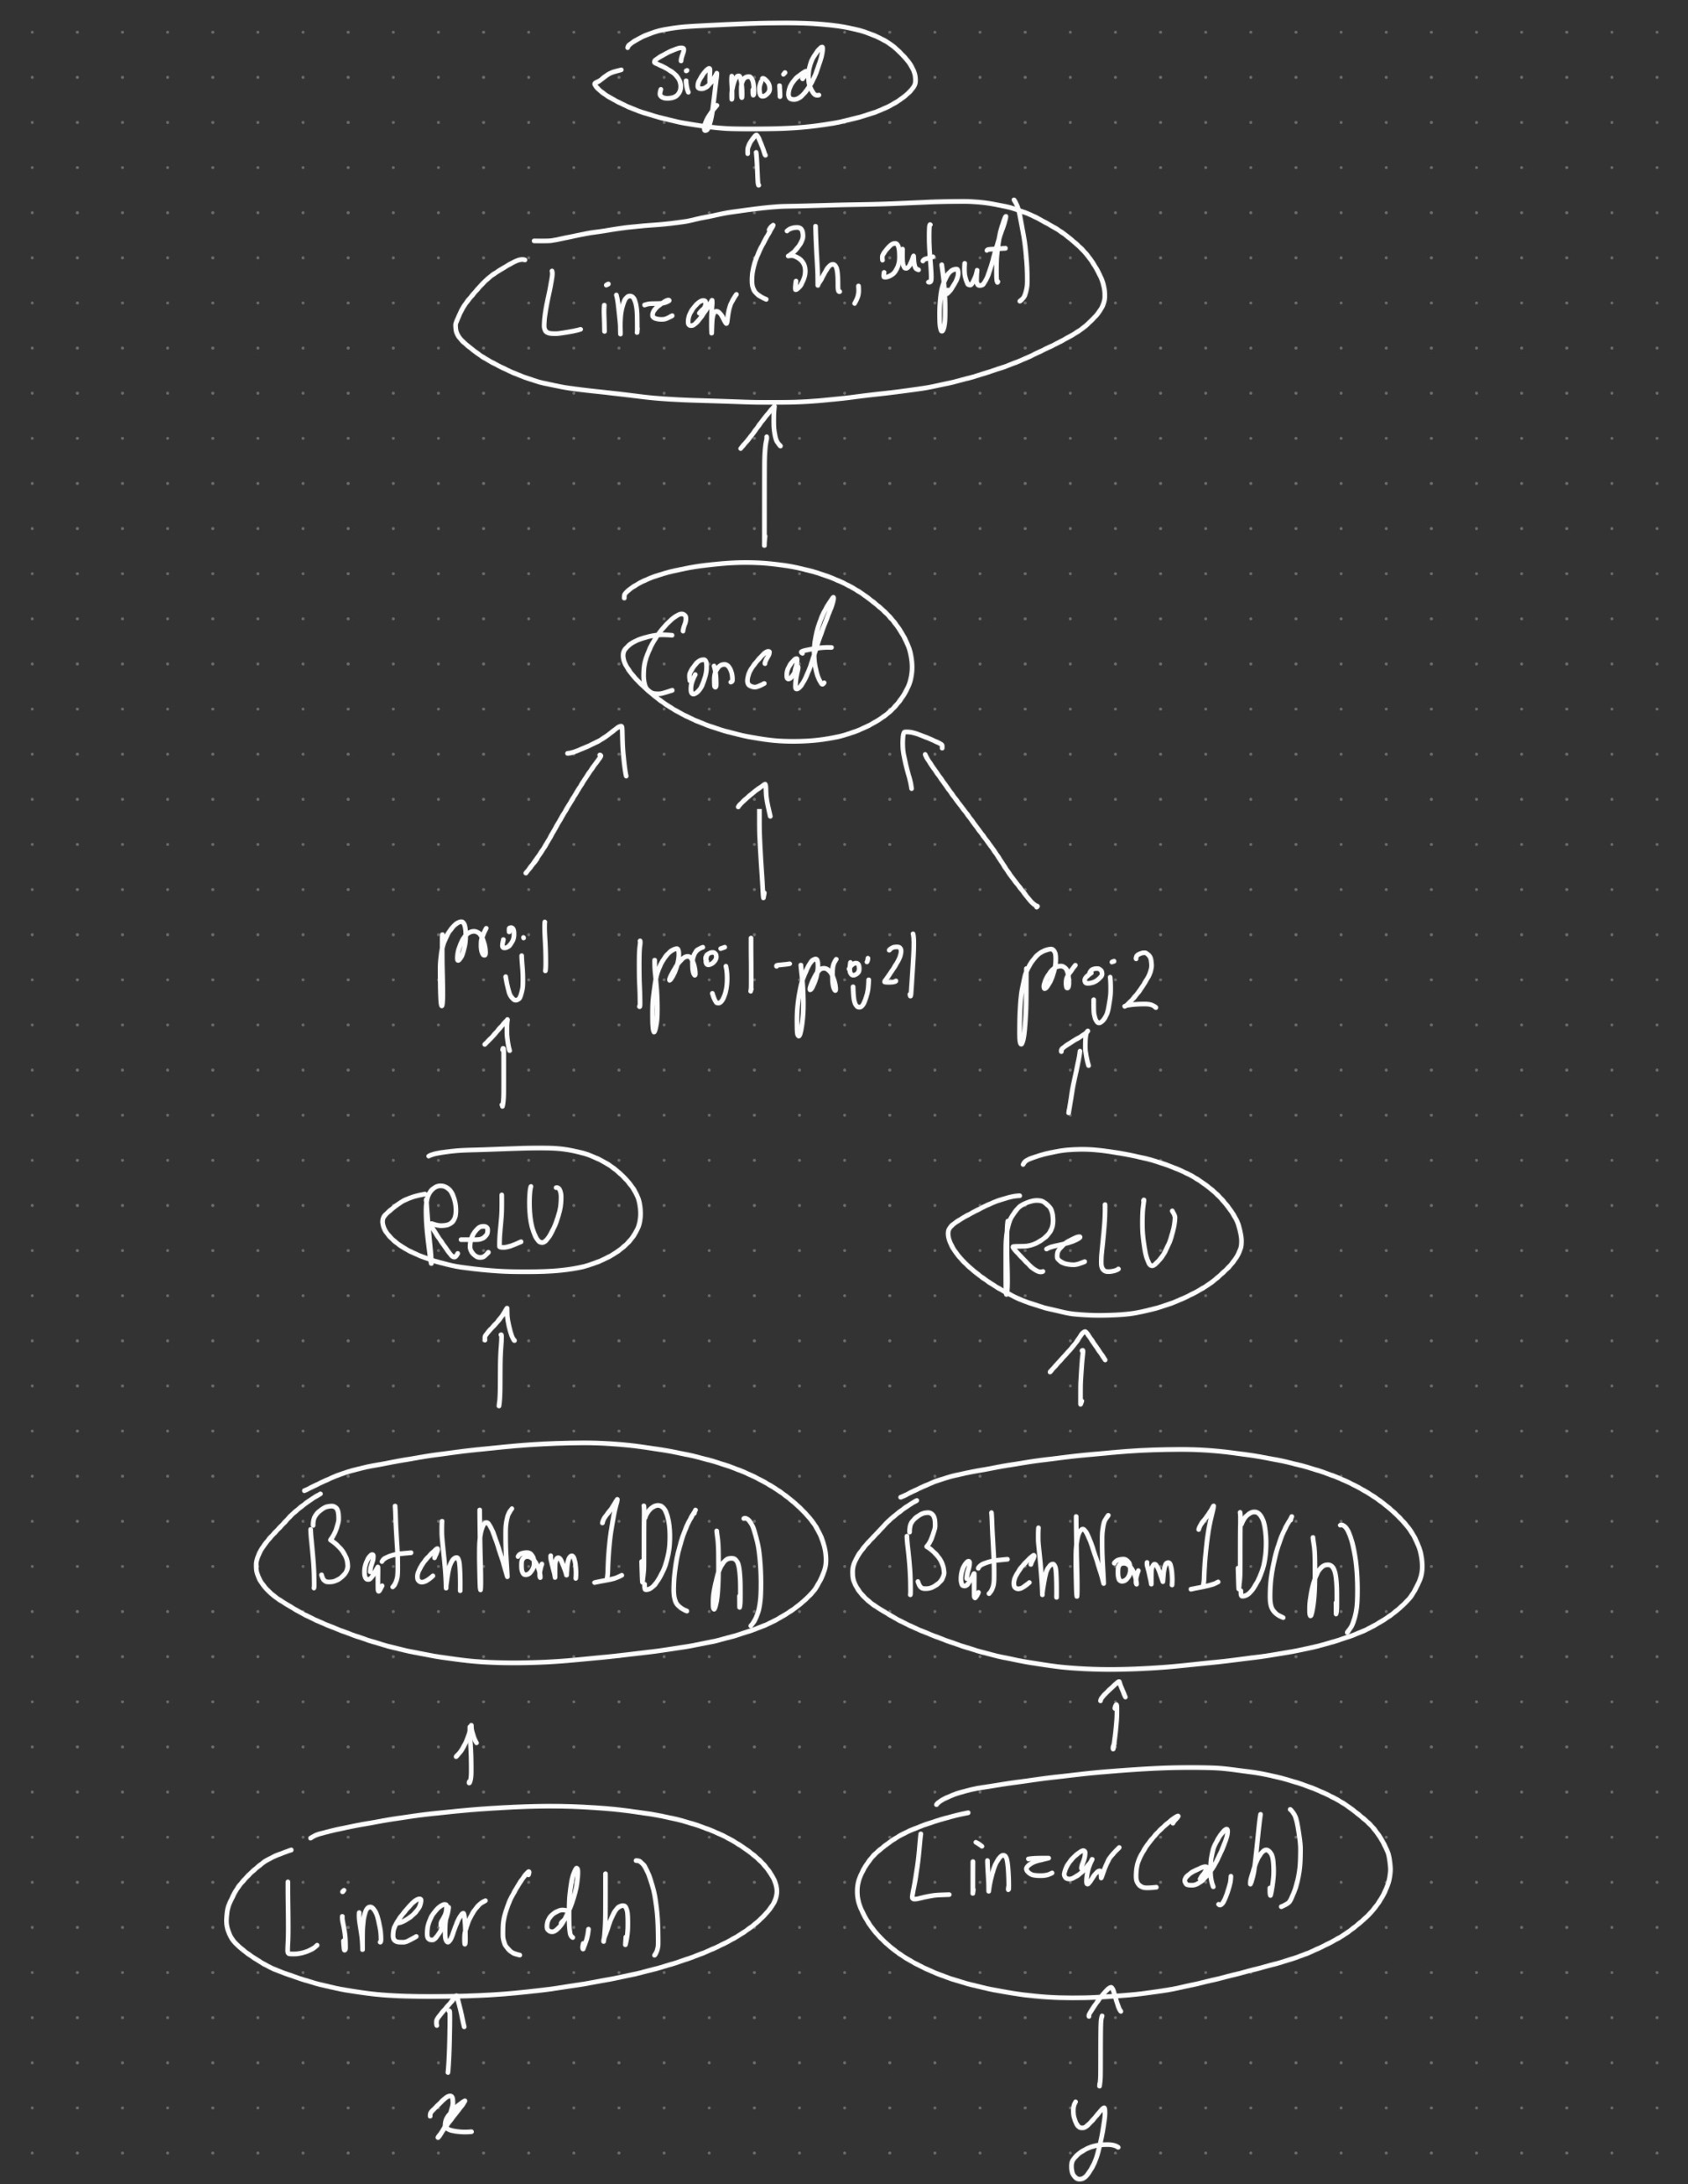
\includegraphics[width=0.8\textwidth]{images/nn_architecture.jpg}
            \caption{Siamese Neural Network}
        \end{figure}
        With higher layer count, you just add another Linear(h,h), BatchNorm1D(h), and ReLU layer after the first one, before calling concat. 

        I chose this model because I felt that the Siamese FFNN architecture would work well since this is inherently a test of similarity. On the website, it says you can use either accuracy or f1 score as the evaluation metric, but I checked and it turns out that 66\% of examples are 1, so the model ended up learning to get a 66\% accuracy by just always guessing 1. So, I wanted to basically maximize precision, so I used f1 score instead. Since 66\% of examples are 1, I realized that I needed to do something to offset this huge bias. I experimented with three ideas: a weighted BCE function, weighted sampling, and batch normalization after each layer. In the end the batch normalization worked best and that is the only one I used. 

        Depth is kind of all over the place with this model, as you can see here (this is only for the sentence transformer embeddings embeddings):
        \begin{figure}[H]
            \centering
            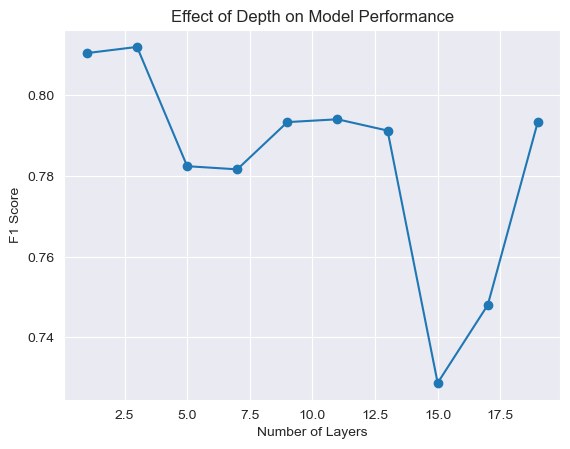
\includegraphics[width=0.8\textwidth]{images/depth_on_siamese.png}
            \caption{Depth vs F1 Score}
        \end{figure}

        I tested the following hyperparameters, with random search, for both GLOVE and Sentence transformer:
        \begin{itemize}
            \item Hidden dimension: 128, 256, 512, 1024, 2048
            \item Number of layers: 1, 2, 3, 4
            \item Learning rate: 1e-5, 1e-4, 1e-3, 1e-2, 1e-1
            \item Number of epochs: 5, 10, 15
            \item batch sizes: 32, 64, 128
        \end{itemize}
        I ended with the following hyperparameters for the GLOVE embeddings:
        \begin{itemize}
            \item Hidden dimension: 512
            \item Number of layers: 2
            \item Learning rate: 1e-4
            \item Number of epochs: 10
            \item batch size: 128
        \end{itemize}
        and this is for the sentence embeddings:
        \begin{itemize}
            \item Hidden dimension: 2048
            \item Number of layers: 1
            \item Learning rate: 1e-3
            \item Number of epochs: 10
            \item batch size: 128
        \end{itemize}
        For the model with sentence transformers, on the test set this gives an accuracy of 74\%, and an f1 score of 82\%, precision of 78\%, and recall of 86\%. I am very happy that this model was able to do very well on precision. 

        On the other hand, for the GLOVE model, the accuracy was 72\%, f1 score of 80\%, precision of 73\%, and recall of 90\%, which is still pretty good. It is curious that the recall is so much higher on this model than with sentence transformers. I personally think this is because the Glove model has an input dim of only 50 vs the sentence transformer who has a dimension of 768. 

        The idea behind this dataset is if two sentences are describing the same event. I have a friend whose username is Meowucme, so I checked if the sentences: ``I saw meow at the store yesterday'' and ``Then I'll meet Meow will venture to the market tomorrow'' were paraphrases, and the model said they weren't, which is correct. 
    \end{enumerate}
\end{document}